\section{Instructions to run the code.} \label{T4}

\paragraph{}The script needs to be run and should run correctly on any linux environment. However, it has only been tested on Debian and WSL environments. The pre-requisite to run the script is to have git, pip3, python3, aws and docker installed. The lightweight script can be downloaded using the following command: \verb|wget https://github.com/antoine-lombardo/log8415-project/releases/download/v1/|\\\verb|script.sh| To make sure the script is executable, the command \verb|sudo chmod +x script.sh| must be executed. The bash script can then be run as root with the command \verb|sudo ./script.sh|. The git repository will then be automatically cloned and the \verb|interactive_deploy.sh| script will be executed, which will automatically install all the necessary Python libraries.

\paragraph{}Alternatively, the script can be run manually. To do so, the repository must be cloned using this command:\\\verb|git clone https://github.com/antoine-lombardo/log8415-project.git|. The script will then be located in the directory \verb|log8415-project/deployment|. The script must be set as executable using the command \verb|sudo chmod +x interactive_deploy.sh|, and can then be run using the command \verb|sudo ./interactive_deploy.sh|.

\paragraph{}When running the script, you'll be asked to setup AWS credentials. If this is your first time using the script, you'll have to do this setup. After that, this step can be omitted, as it will fetch the default credentials saved in AWS.\\

\begin{figure}[htbp]
  \centering
  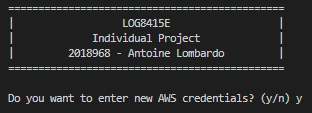
\includegraphics[width=7cm]{Resources/script_1.png}
  \caption{Execution of the command sudo ./script.sh}
\end{figure}\\

\paragraph{}When AWS configuration is done, you'll be asked what action needs to be done. For this project, there is only one option, which is to deploy the system.

\begin{figure}[htbp]
  \centering
  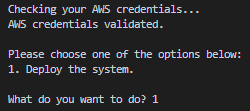
\includegraphics[width=7cm]{Resources/script_2.png}
  \caption{Action selection}
\end{figure}

\paragraph{}The deployment will then star:.

\begin{figure}[htbp]
  \centering
  \begin{minipage}[b]{0.44\textwidth}
    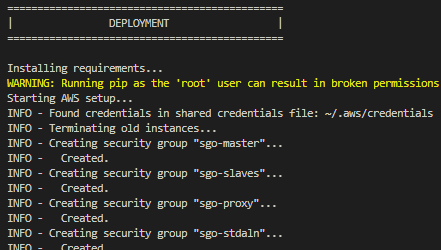
\includegraphics[height=4cm]{Resources/script_3.png}
    \caption{Start of the deployment}
  \end{minipage}
  \hfill
  \begin{minipage}[b]{0.54\textwidth}
    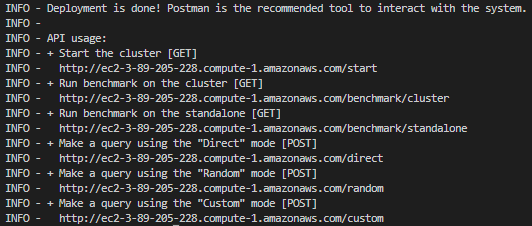
\includegraphics[height=4cm]{Resources/script_4.png}
    \caption{End of the deployment}
  \end{minipage}
\end{figure}\\

\paragraph{}The user can then interact with the REST API using any tools such as Postman. For Postman, a Collection has been included in the Github repository which gives access to all the functions of the system. Please note that the Cluster need to be start prior any other actions.

\begin{figure}[htbp]
  \centering
  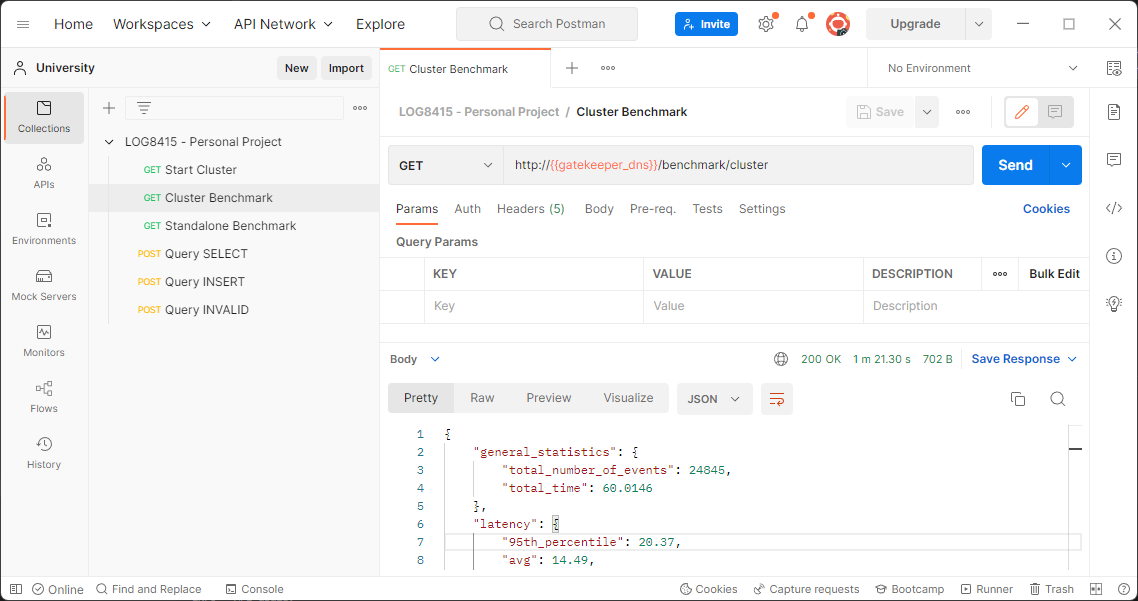
\includegraphics[width=14cm]{Resources/postman.png}
  \caption{Postman interface}
\end{figure}\\


